\documentclass[conference]{IEEEtran}
\IEEEoverridecommandlockouts
% The preceding line is only needed to identify funding in the first footnote. If that is unneeded, please comment it out.
%Template version as of 6/27/2024
\usepackage{hyperref}
\usepackage{cite}
\usepackage{amsmath,amssymb,amsfonts}
\usepackage{amsmath, amssymb}
\usepackage{graphicx}
\usepackage{booktabs}
\usepackage{siunitx}
\usepackage{tikz}
\usepackage[american]{circuitikz}
\usetikzlibrary{calc}
\sisetup{per-mode=symbol}

\usepackage{algorithmic}
\usepackage{graphicx}
\usepackage{textcomp}
\usepackage{xcolor}
\def\BibTeX{{\rm B\kern-.05em{\sc i\kern-.025em b}\kern-.08em
    T\kern-.1667em\lower.7ex\hbox{E}\kern-.125emX}}
\begin{document}

\title{Progetto Electromagnetic Materials}

\author{\IEEEauthorblockN{1\textsuperscript{st} Matteo Fiaschi}
}


\maketitle

\begin{abstract}
In questo report sono riportati i risultati risultanti dal lavoro svolto sul progetto $\#5$
\end{abstract}


\section{Introduzione}
Il sensore analizzato consiste in una metasuperficie stampata su substrato dielettrico  (\(\varepsilon_r = 4.4\), spessore \(d = \SI{2}{mm}\)), modellata come un circuito RLC serie. La capacità del sistema varia con l'umidità secondo una relazione lineare o cubica. Gli obiettivi principali sono:
\begin{itemize}
    \item Calcolare la risposta in frequenza del coefficiente di riflessione (\(\Gamma\)) attorno a \(\SI{2.5}{GHz}\),
    \item Determinare la curva di calibrazione per i casi lineare/cubico,
    \item Valutare l'impatto del rumore sulle prestazioni del sensore.
\end{itemize}


\section{Teoria}
\subsection{Modello Circuitale RLC Serie}
La metasuperficie è rappresentata da un circuito RLC serie con impedenza:
\begin{equation}
    Z_{\text{RLC}} = R + j\omega L + \frac{1}{j\omega C} = R + j\left(\omega L - \frac{1}{\omega C}\right),
\end{equation}
dove:
\begin{itemize}
    \item \(R \): Resistenza parassita,
    \item \(L \): Induttanza equivalente,
    \item \(C(H)\): Capacità dipendente dall'umidità \(H\).
\end{itemize}

\subsection{Accoppiamento con il Substrato}
L'impedenza del substrato dielettrico, modellata come linea di trasmissione, è:
\begin{equation}
    Z_{\text{sub}} = Z_d \frac{Z_d + jZ_0 \tan(\beta d)}{Z_0 + jZ_d \tan(\beta d)},
\end{equation}
dove:
\begin{itemize}
    \item \(Z_d = \sqrt{\mu_0/(\varepsilon_0 \varepsilon_r)} \approx \SI{177.5}{\ohm}\),
    \item \(\beta = \omega\sqrt{\mu_0 \varepsilon_0 \varepsilon_r}\): Costante di fase,
    \item \(Z_0 = \SI{377}{\ohm}\): Impedenza del vuoto.
\end{itemize}

\begin{figure}[ht!]
    \centering
    \begin{circuitikz}[scale=1.2, european resistors]
        % RLC serie
        \draw (1,1) to[short, o-] (0,1)
              to[R, l=$R$] (0,3)
              to[L, l=$L$] (0,5)
              to[C, l=$C$, *-*] (0,7)
              to[short, -o] (1,7);
        % Substrato in parallelo
        \draw (0,1) to[short] (-2,1) 
              to[generic, l=$Z_{\text{sub}}$, -*] (-2,7)
              to[short] (0,7);
        % Etichette
        \draw[->] (3,4) -- node[above]{Onda incidente} (2,4);
        \draw (0,4) node[right]{$Z_0 = \SI{377}{\ohm}$};
    \end{circuitikz}
    \caption{Modello circuitale corretto: RLC serie in parallelo con l'impedenza del substrato.}
    \label{fig:circuito}
\end{figure}

\subsection{Relazione Capacità-Umidità}
\begin{itemize}
    \item \textbf{Caso Lineare }: 
    \[
    C(H) = C_0 (1 + \alpha H), \quad \alpha = \text{costante di sensibilità}
    \]
    \item \textbf{Caso Cubico }: 
    \[
    C(H) = C_0 (1 + \beta H^3), \quad \beta = \text{costante non lineare}
    \]
\end{itemize}

\subsection{Coefficiente di Riflessione}
L'impedenza totale è il parallelo tra \(Z_{\text{RLC}}\) e \(Z_{\text{sub}}\):
\[
Z_{\text{tot}} = \frac{Z_{\text{RLC}} \cdot Z_{\text{sub}}}{Z_{\text{RLC}} + Z_{\text{sub}}}
\]
Il coefficiente di riflessione è:
\[
\Gamma = \frac{Z_{\text{tot}} - Z_0}{Z_{\text{tot}} + Z_0}
\]

%======================================================================
\section{Risultati e Discussione}
\subsection{Parametri di Simulazione}
\begin{itemize}
    \item Frequenza: \(\SIrange{1}{5}{GHz}\),
    \item Parametri RLC: \(R = \SI{1}{\ohm},\ L = \SI{94}{nH},\ C_0 = \SI{43.1}{fF}\),
    \item Variazione di \(C\): \(0 \to + 50\%\).
\end{itemize}

\subsection{Risposta in Frequenza}
Siccome $ d \ll \lambda/n_r$ allora per le relazioni di dispersione $\beta d \ll 1$, ciò significa che in prima approssimazione $Z_{sub} \simeq \frac{Z_d^2}{Z_0}$. Questo significa che  la frequenza di risonanza, $Z_{sub}$ sarà solo un termine aggiuntivo da aggiungere alla parte resistiva, che sarà importante in quanto modifica il fattore di qualità $Q$. La scelta dei parametri sovrariportati ha tenuto conto anche del fatto appena discusso.
\begin{figure}[ht!]
    \centering
    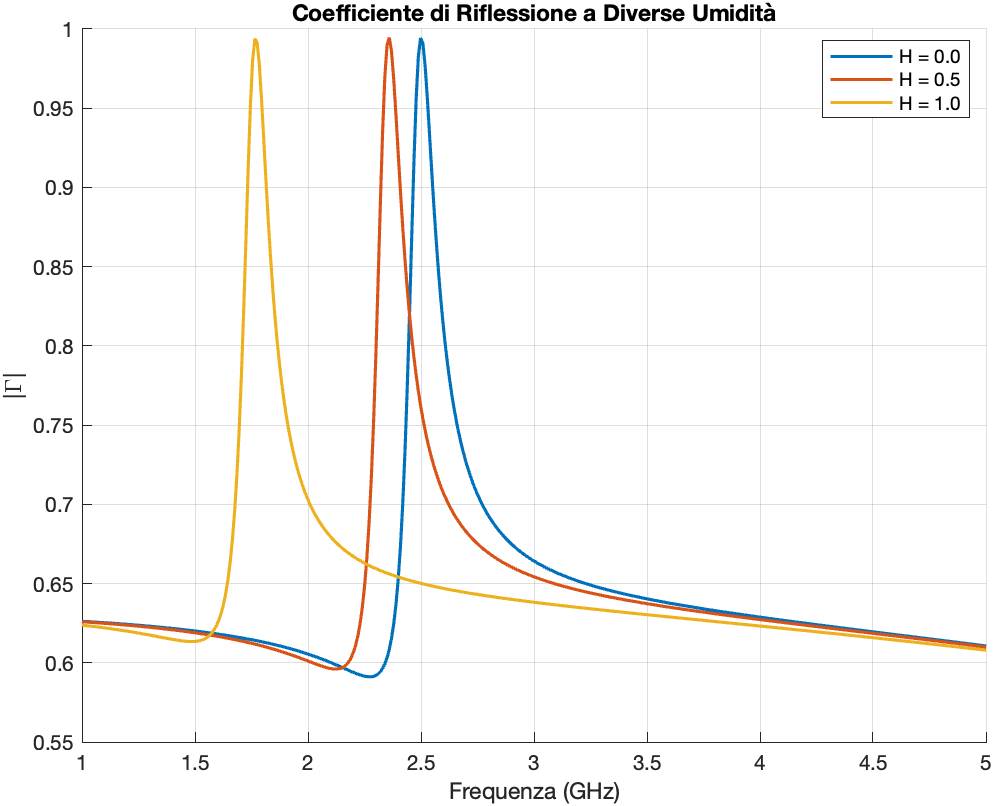
\includegraphics[width=0.5\textwidth]{img/grafici.png}
    \caption{Andamento di \(|\Gamma|\) per variazione cubica di \(C\). }
    \label{fig:gamma}
\end{figure}

\subsection{Curve di Calibrazione}
Imponendo la condizione di risonanza a $Z_{RLC}$ otteniamo che la frequenza di risonanza nei due casi può essere espressa come:


\begin{itemize}
    \item \textbf{Caso Lineare}:
    \[
    f_{\text{res}}(H) = \frac{1}{2\pi\sqrt{L C_0 (1 + \alpha H)}} \approx f_0 \left(1 - \frac{\alpha H}{2}\right)
    \]
    \item \textbf{Caso Cubico}:
    \[
    f_{\text{res}}(H) = \frac{f_0}{\sqrt{1 + \beta H^3}} \approx f_0 \left(1 - \frac{\beta H^3}{2}\right)
    \]
\end{itemize}
Per $\alpha,\beta$ piccoli le espressioni possono essere approssimate. Ci aspettiamo che la di risonanza vari rispettivamente in modo lineare e in modo cubico rispetto all'umidità. Già da questa analisi qualitativa possiamo intuire che il sensore che varia linearmente sarà migliore in climi secchi mentre altri in quelli umidi\footnote{Questo è certamente vero per $\beta = \alpha^3$}
\begin{figure}[h!]
    \centering
    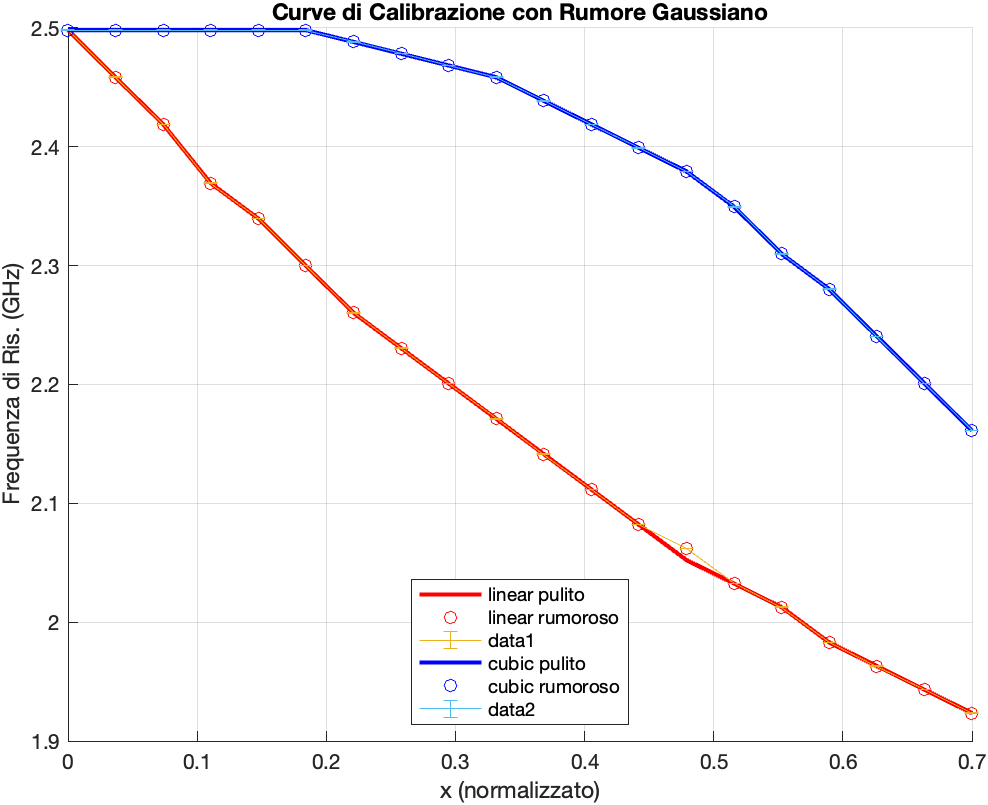
\includegraphics[width=0.5\textwidth]{img/curve.png}
    \caption{Andamento di \(|\Gamma|\) per variazione cubica di \(C\). }
    \label{fig:curve}
\end{figure}
\subsection{Analisi del Rumore}
Con rumore gaussiano 30 dB, non sono state ottenute effettive differenze tra i valori di H senza e con il rumore. Nel codice è stato implementato un sistema per il calcolo di quest ultimo ma come si può notare in \autoref{fig:curve}, i grafici con rumore stanno nelle barre di errore.
\begin{figure}[!ht]
    \centering
    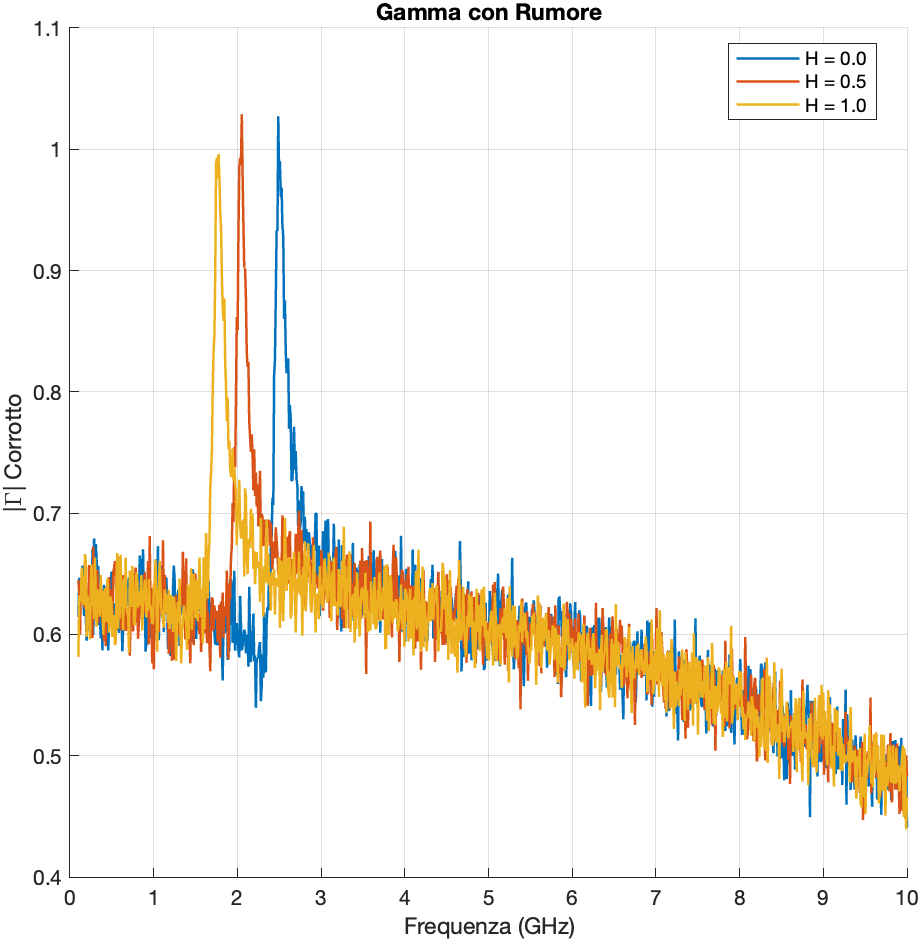
\includegraphics[width=\linewidth]{img/rumore.png}
    \caption{$\Gamma $ corrotto con rumore bianco, SNR 30 dB}
    \label{fig:rumore}
\end{figure}
%======================================================================
\section{Conclusioni}
Il sensore presenta:
\begin{itemize}
    \item Alta sensibilità  lineare (\(\Delta f/\Delta H \approx \SI{12.5}{MHz/\%RH}\)),
    
    \item Robustezza alle interferenze grazie alla risonanza acuta (\(Q_{RLC} \approx 1500\)).
\end{itemize}
Raccomandazioni:
\begin{itemize}
    \item Utilizzare materiali a bassa perdita per migliorare \(Q_{RLC} = \sqrt{\frac{L}{CR^2}}\),
    
\end{itemize}

\end{document}